% ═════════════════════════════════════════════════════════════════════════════
\chapter{Teoria dei Computer Quantistici}
\label{chap:quantum}
% ═════════════════════════════════════════════════════════════════════════════

% ─────────────────────────────────────────────────────────────────────────────
\section{Introduzione al Paradigma Quantistico}
\label{sec:intro}
% ─────────────────────────────────────────────────────────────────────────────

Negli ultimi decenni, il progresso nell'elaborazione delle informazioni ha
seguito la celebre \textit{Legge di Moore}, che descrive il raddoppio
approssimativo del numero di transistor per chip ogni due anni. Tuttavia,
man mano che le dimensioni dei componenti elettronici si avvicinano alla scala
atomica, i limiti fisici della computazione classica diventano sempre più
evidenti. In questo contesto emerge il paradigma della \textbf{computazione
quantistica}, che sfrutta i principi della meccanica quantistica ---
sovrapposizione, entanglement e interferenza --- per elaborare le informazioni
in modo radicalmente diverso rispetto ai computer tradizionali~\cite{nielsen2010quantum}.

Un computer classico elabora le informazioni attraverso \textit{bit} binari, che
possono assumere i valori $0$ o $1$. Al contrario, un computer quantistico
utilizza i \textbf{qubit} (\textit{quantum bit}), che grazie al principio di
sovrapposizione possono esistere contemporaneamente in una combinazione di
$\ket{0}$ e $\ket{1}$ fino al momento della misurazione. Questa proprietà,
combinata con l'entanglement quantistico e le operazioni di interferenza,
conferisce ai computer quantistici un potenziale computazionale enormemente
superiore per determinate classi di problemi.

% ─────────────────────────────────────────────────────────────────────────────
\section{Fondamenti Teorici della Computazione Quantistica}
\label{sec:fondamenti}
% ─────────────────────────────────────────────────────────────────────────────

\subsection{Il Qubit e la Sovrapposizione Quantistica}
\label{subsec:qubit}

\begin{definizione}[Qubit]
  Un \textbf{qubit} è il sistema fisico a due livelli che costituisce l'unità
  fondamentale di informazione nella computazione quantistica. Il suo stato puro
  è descritto da un vettore nello spazio di Hilbert $\mathcal{H} \cong \mathbb{C}^2$:
  \begin{equation}
    \ket{\psi} = \alpha\ket{0} + \beta\ket{1}, \qquad
    \alpha, \beta \in \mathbb{C}, \quad |\alpha|^2 + |\beta|^2 = 1.
    \label{eq:qubit}
  \end{equation}
\end{definizione}

I coefficienti $\alpha$ e $\beta$ sono le \textit{ampiezze di probabilità}: una
misurazione restituisce $0$ con probabilità $|\alpha|^2$ e $1$ con probabilità
$|\beta|^2$, collassando lo stato in uno dei due vettori base. Geometricamente,
ogni stato puro di un qubit corrisponde a un punto sulla superficie della
\textbf{sfera di Bloch} (Figura~\ref{fig:bloch}), parametrizzata da:
\begin{equation}
  \ket{\psi} = \cos\frac{\theta}{2}\ket{0} + e^{i\varphi}\sin\frac{\theta}{2}\ket{1},
  \qquad \theta \in [0,\pi],\ \varphi \in [0, 2\pi).
\end{equation}

\begin{figure}[ht]
  \centering
  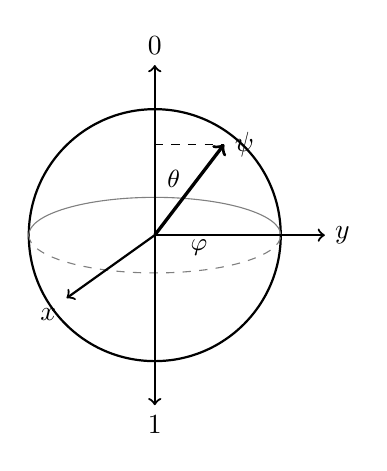
\begin{tikzpicture}[scale=1.6]
    \draw[thick] (0,0) circle (1);
    \draw[dashed, gray] (-1,0) arc (180:360:1 and 0.3);
    \draw[gray] (-1,0) arc (180:0:1 and 0.3);
    \draw[->, thick] (0,0) -- (0,1.35) node[above] {$\ket{0}$};
    \draw[->, thick] (0,0) -- (0,-1.35) node[below] {$\ket{1}$};
    \draw[->, thick] (0,0) -- (1.35,0) node[right] {$y$};
    \draw[->, thick] (0,0) -- (-0.7,-0.5) node[below left] {$x$};
    \draw[->, very thick] (0,0) -- (0.55,0.72) node[right] {$\ket{\psi}$};
    \draw[dashed] (0,0.72) -- (0.55,0.72);
    \draw[dashed] (0,0) -- (0.55,0.72);
    \node at (0.15, 0.45) {\small $\theta$};
    \node at (0.35,-0.1) {\small $\varphi$};
  \end{tikzpicture}
  \caption{Rappresentazione geometrica di un qubit sulla sfera di Bloch.
    I poli nord e sud corrispondono agli stati base $\ket{0}$ e $\ket{1}$.}
  \label{fig:bloch}
\end{figure}

\subsection{L'Entanglement Quantistico}
\label{subsec:entanglement}

\begin{principio}[Entanglement]
  Due qubit si dicono \textbf{entangled} (intrecciati) se il loro stato
  composto $\ket{\Psi} \in \mathcal{H}^{\otimes 2}$ non è fattorizzabile come
  prodotto tensoriale degli stati individuali:
  $\ket{\Psi} \neq \ket{\psi_1} \otimes \ket{\psi_2}$.
\end{principio}

Il prototipo di stato entangled è fornito dalla base degli \textbf{stati di Bell}:
\begin{align}
  \ket{\Phi^+} &= \frac{1}{\sqrt{2}}\bigl(\ket{00} + \ket{11}\bigr), &
  \ket{\Phi^-} &= \frac{1}{\sqrt{2}}\bigl(\ket{00} - \ket{11}\bigr), \\
  \ket{\Psi^+} &= \frac{1}{\sqrt{2}}\bigl(\ket{01} + \ket{10}\bigr), &
  \ket{\Psi^-} &= \frac{1}{\sqrt{2}}\bigl(\ket{01} - \ket{10}\bigr).
\end{align}

L'entanglement è la risorsa centrale di algoritmi e protocolli quantistici
fondamentali quali la teletrasportazione quantistica, la distribuzione
quantistica delle chiavi (\textit{QKD}) e il \textit{dense coding}.
Einstein definì il fenomeno con l'espressione \textit{``spooky action at a
distance''}, ritenendolo incompatibile con il realismo locale; le disuguaglianze
di Bell~(1964) e le successive verifiche sperimentali hanno confutato tale ipotesi.

\subsection{Le Porte Logiche Quantistiche}
\label{subsec:porte}

La computazione quantistica si effettua tramite \textbf{porte logiche
quantistiche}, ovvero trasformazioni unitarie $U \in \mathrm{U}(2^n)$ applicate
a registri di $n$ qubit. A differenza delle porte classiche, ogni operazione
quantistica (eccetto la misurazione) è \textit{reversibile}.
Le porte più importanti su singolo qubit sono:
\begin{equation}
  H = \frac{1}{\sqrt{2}}\begin{pmatrix}1 & 1 \\ 1 & -1\end{pmatrix}, \quad
  X = \begin{pmatrix}0 & 1 \\ 1 & 0\end{pmatrix}, \quad
  T = \begin{pmatrix}1 & 0 \\ 0 & e^{i\pi/4}\end{pmatrix}.
\end{equation}

La porta a due qubit \textbf{CNOT} è definita da:
\begin{equation}
  \mathrm{CNOT} = \begin{pmatrix}1&0&0&0\\0&1&0&0\\0&0&0&1\\0&0&1&0\end{pmatrix}.
\end{equation}

L'insieme $\{H, T, \mathrm{CNOT}\}$ è \textit{universale}: ogni trasformazione
unitaria può essere approssimata con precisione arbitraria da una composizione
finita di queste porte (teorema di Solovay--Kitaev)~\cite{nielsen2010quantum}.
Un esempio di circuito per generare lo stato di Bell $\ket{\Phi^+}$ è mostrato
di seguito:
\begin{center}
\begin{quantikz}
  \lstick{$\ket{0}$} & \gate{H} & \ctrl{1} & \rstick[2]{$\ket{\Phi^+}$} \\
  \lstick{$\ket{0}$} & \qw      & \targ{}  &
\end{quantikz}
\end{center}

% ─────────────────────────────────────────────────────────────────────────────
\section{Vantaggi dei Computer Quantistici}
\label{sec:vantaggi}
% ─────────────────────────────────────────────────────────────────────────────

Il vantaggio computazionale dei sistemi quantistici si manifesta in specifiche
classi di problemi dove gli algoritmi quantistici offrono un'accelerazione
\textit{esponenziale} o \textit{polinomiale} rispetto ai migliori algoritmi
classici noti.

\begin{itemize}
  \item \textbf{Fattorizzazione e crittografia.}
    L'\textbf{algoritmo di Shor}~\cite{shor1994algorithms} fattorizza un intero
    $N$ in tempo polinomiale $O((\log N)^3)$, con implicazioni dirette sulla
    sicurezza dei sistemi crittografici RSA e ElGamal.

  \item \textbf{Ricerca non strutturata.}
    L'\textbf{algoritmo di Grover}~\cite{grover1996fast} individua un elemento in
    un database non strutturato di $N$ voci in $O(\sqrt{N})$ valutazioni
    dell'oracolo, ottenendo uno \textit{speedup} quadratico rispetto alla ricerca
    classica $O(N)$.

  \item \textbf{Simulazione quantistica.}
    Feynman~\cite{feynman1982simulating} osservò che i sistemi quantistici sono
    naturalmente simulati da computer quantistici. La simulazione di molecole con
    precisione quantomeccanica, esponenzialmente costosa classicamente, è
    affrontabile efficientemente su hardware quantistico.

  \item \textbf{Ottimizzazione combinatoria.}
    Algoritmi come QAOA (\textit{Quantum Approximate Optimization Algorithm}) e
    il \textit{Quantum Annealing} offrono approcci promettenti per problemi
    NP-difficili in logistica, finanza e machine learning.

  \item \textbf{Crittografia quantistica.}
    Il protocollo BB84~\cite{bennett1984bb84} garantisce la sicurezza
    informazione-teorica della distribuzione delle chiavi: qualsiasi tentativo
    di intercettazione altera irreversibilmente gli stati trasmessi.
\end{itemize}

% ─────────────────────────────────────────────────────────────────────────────
\section{Limiti e Sfide dei Computer Quantistici}
\label{sec:limiti}
% ─────────────────────────────────────────────────────────────────────────────

Nonostante il loro potenziale, i computer quantistici presentano sfide tecniche
e teoriche che ne limitano attualmente l'applicabilità pratica su larga scala.

\begin{itemize}
  \item \textbf{Decoerenza quantistica.}
    I qubit sono estremamente sensibili alle perturbazioni ambientali. I tempi di
    coerenza $T_1$ (rilassamento) e $T_2$ (sfasamento) nei qubit superconduttori
    tipici sono dell'ordine di $10$--$500\,\mu$s, limitando la profondità dei
    circuiti eseguibili.

  \item \textbf{Correzione degli errori quantistici.}
    I codici di correzione degli errori (codice di superficie, codice di Steane)
    richiedono un overhead di $10^3$--$10^4$ qubit fisici per qubit logico
    affidabile~\cite{preskill2018quantum}. I sistemi attuali operano in regime
    NISQ (\textit{Noisy Intermediate-Scale Quantum}), privi di correzione
    completa.

  \item \textbf{Scalabilità hardware.}
    I processori superconduttori richiedono temperature criogeniche $\sim
    15\,\text{mK}$. Le tecnologie alternative (qubit fotonici, trappole ioniche,
    qubit topologici) presentano diversi compromessi tra coerenza, fedeltà e
    scalabilità.

  \item \textbf{Programmabilità e stack software.}
    I framework attuali (Qiskit, Cirq, PennyLane) stanno maturando, ma la
    distanza rispetto all'accessibilità della programmazione classica rimane ampia.

  \item \textbf{Applicabilità circoscritta.}
    Per la grande maggioranza dei compiti computazionali --- elaborazione di testi,
    database relazionali, navigazione web --- i computer classici rimangono più
    efficienti e pratici.
\end{itemize}

\begin{notabox}
  Il concetto di \textit{quantum advantage} si riferisce alla dimostrazione che
  un dispositivo quantistico risolve un problema specifico più velocemente di
  qualsiasi computer classico noto. La sua dimostrazione sperimentale su problemi
  di rilevanza pratica rimane una delle sfide aperte più importanti del settore.
\end{notabox}

% ─────────────────────────────────────────────────────────────────────────────
\section{Confronto Sistemico: Classico vs.\ Quantistico}
\label{sec:confronto}
% ─────────────────────────────────────────────────────────────────────────────

La Tabella~\ref{tab:confronto} sintetizza le principali differenze tra le due
architetture computazionali.

\begin{table}[ht]
  \centering
  \renewcommand{\arraystretch}{1.3}
  \caption{Confronto tra computer classici e computer quantistici.}
  \label{tab:confronto}
  \begin{tabularx}{\textwidth}{>{\bfseries}lXX}
    \toprule
    Caratteristica      & Computer Classico               & Computer Quantistico \\
    \midrule
    Unità base          & Bit ($0$ o $1$)                 & Qubit ($\ket{0}$, $\ket{1}$, sovrapposizione) \\
    Operazioni          & Porte irreversibili              & Trasformazioni unitarie reversibili \\
    Parallelismo        & Sequenziale / multicore          & Parallelismo quantistico ($2^n$ ampiezze) \\
    Gestione errori     & Matura e affidabile              & In sviluppo (QEC, regime NISQ) \\
    Condizioni operative & Temperatura ambiente            & Criogenica ($\sim 15\,\text{mK}$) \\
    Applicazioni ottimali & Uso generale, I/O, database   & Crittografia, simulazione, ottimizzazione \\
    Maturità tecnologica & Estremamente matura             & Emergente \\
    Costi               & Accessibili, scala industriale  & Elevati, infrastruttura specializzata \\
    \bottomrule
  \end{tabularx}
\end{table}

% ─────────────────────────────────────────────────────────────────────────────
\section{Stato dell'Arte e Prospettive Future}
\label{sec:stato}
% ─────────────────────────────────────────────────────────────────────────────

Nel 2019, Google ha raggiunto la \textbf{supremazia quantistica} con il
processore \textit{Sycamore} da 53 qubit~\cite{arute2019quantum}, completando
in $\sim 200\,\text{s}$ un campionamento casuale di circuiti che richiederebbe
stimativamente $10\,000$ anni al supercomputer \textit{Summit}. Tale
affermazione è stata contestata da IBM, che ha proposto algoritmi classici più
efficienti per lo stesso problema.

Nel 2023, IBM ha presentato il processore \textbf{Condor} da $1\,121$ qubit,
mentre Microsoft ha accelerato lo sviluppo dei qubit topologici basati sui
fermioni di Majorana. Il modello di accesso dominante si sta spostando verso il
paradigma \textbf{cloud}: IBM Quantum Network, AWS Braket, Google Quantum AI e
Azure Quantum offrono accesso remoto a processori reali.

Il percorso più realistico per le applicazioni nei prossimi anni è il paradigma
\textbf{ibrido classico-quantistico}, in cui il computer quantistico funge da
co-processore acceleratore per specifici sottoproblemi, mentre il controllo
generale rimane classico~\cite{preskill2018quantum}.

% ─────────────────────────────────────────────────────────────────────────────
\section{Conclusioni del Capitolo}
\label{sec:conclusioni}
% ─────────────────────────────────────────────────────────────────────────────

La computazione quantistica rappresenta un cambio di paradigma fondamentale,
non una semplice evoluzione incrementale dei sistemi classici. I suoi vantaggi
teorici --- accelerazione esponenziale per la fattorizzazione, ricerca,
simulazione e ottimizzazione --- sono matematicamente dimostrati. Tuttavia, la
distanza tra teoria e implementazione hardware rimane considerevole: la
decoerenza, gli errori fisici e le difficoltà di scalabilità costituiscono
ostacoli tecnici genuini e non ancora risolti.

Il futuro prevedibile non vede i computer quantistici \textit{sostituire} quelli
classici, bensì \textit{affiancarli} in architetture ibride specializzate.
I capitoli successivi analizzeranno in dettaglio le architetture hardware
esistenti, gli algoritmi quantistici più rilevanti e le prospettive applicative
nei settori della crittografia, della farmacologia computazionale e
dell'intelligenza artificiale.
